% !TEX root = saveliev_physics_general_course_1.tex
%!TEX TS-program = pdflatex
%!TEX encoding = UTF-8 Unicode

%\chapter{THE CRYSTALLINE STATE}\label{chap:13}
 
\chapter{TRẠNG THÁI KẾT TINH}\label{chap:13}

%\section{Features of the Crystalline State}\label{sec:13_1}

\section{Những nét đặc trưng của trạng thái kết tinh}\label{sec:13_1}

%The majority of solids in nature have a crystalline structure. For example, almost all minerals and all metals in the solid state are crystals.

Tuyệt đại đa số các chất rắn trong thiên nhiên có cấu tạo tinh thể. Chẳng hạn, hầu hết các khoáng vật và tất cả các kim loại ở trạng thái rắn đều là các tinh thể.

%A feature of the crystalline state distinguishing it from the fluid states is the presence of \textbf{anisotropy}, \ie, the dependence of a number of physical properties (mechanical, thermal, electrical, optical) on the direction.

Nét đặc trưng của trạng thái kết tinh khác với các trạng thái lỏng và khí của nó là ở chỗ nó có \textbf{tính dị hướng}, tức sự phụ thuộc của nhiều tính chất vật lý (cơ học, nhiệt học, điện học, quang học) vào hướng.

%Bodies whose properties are identical in all directions are called \textbf{isotropic}. In addition to gases and, with a few exceptions, all liquids, amorphous solids are also isotropic. These solids are supercooled liquids (see Sec.~\ref{sec:15_6}).

Những chất có những tính chất như nhau theo tất cả mọi hướng gọi là những \textbf{chất đẳng hướng}. Ngoài các chất khí ra thì tất cả các chất lỏng, trừ một vài trường hợp đặc biệt, và cả những chất rắn vô định hình đều là những chất đẳng hướng. Các chất rắn vô định hình là các chất lỏng bị cô đặc (xem phần~\ref{sec:15_6}).

%The reason why crystals are anisotropic is the ordered arrangement of the particles they are built of (atoms or molecules). The ordered arrangement of the particles manifests itself in the regular external facetting of crystals. Crystals are restricted by plane facets making angles with one another characteristic of a given species of crystals. It is easy to split crystals along definite planes called \textbf{cleavage planes}.

Nguyên nhân của sự dị hướng của các tinh thể là sự sắp xếp có trật tự của các hạt (các nguyên tử hoặc phân tử) cấu tạo nên các tinh thể đó. Sự sắp xếp có trật tự của các hạt được thể hiện ở hình dáng cân đối bên ngoài của các tinh thể. Các tinh thể giới hạn vởi các mặt biên phẳng, cắt nhau theo những góc xác định nào đó đối với từng loại tinh thể đã cho. Ta có thể tách dễ dàng các tinh thể theo các mặt phẳng xác định được gọi là các \textbf{mặt phẳng tách}.

%The regularity of the geometrical shape and the anisotropy of crystals do not usually manifest themselves because crystalline bodies are encountered, as a rule, in the form of \textbf{polycrystals}, \ie, conglomerates of a multitude of intergrown, randomly oriented fine crystals. Anisotropy is observed in polycrystals only within the confines of each separately taken minute crystal. A body as a whole does not display anisotropy owing to the chaotic orientation of its crystals. By providing special conditions of crystallization from a melt or a solution, we can obtain large single crystals---\textbf{monocrystals} of any substance. Monocrystals of some minerals are encountered in nature.

Sự cân đối của hình dạng hình học và tính dị hướng của các tinh thể thường không thể hiện ra do ở chỗ là các chất kết tinh mà ta gặp lại hay ở dưới dạng các \textbf{đa tinh thể}, tức là một khối kết tụ của một số rất lớn những tinh thể nhỏ xíu định hướng một cách rối loạn. Trong các đa tinh thể, ta chỉ có thể quan sát được tính dị hướng trong phạm vi của mỗi tinh thể nhỏ tách biệt, còn trong toàn bộ vật ta không phát hiện được tính dị hướng do ở sự định hướng hỗn loạn của các tinh thể nhỏ. Bằng cách tạo ra những điều kiện kết tinh đặc biệt từ các chất rắn nấu chảy hoặc từ các dung dịch, ta có thể thu được những tinh thể đơn lớn là những \textbf{đơn tinh thể} của bất kỳ một chất nào. Trong thiên nhiên, ta thường gặp những đơn tinh thể của một số khoáng vật ở trạng thái tự nhiên.

%The ordered nature of the arrangement of the atoms (or molecules) of a crystal consists in that they are located at the points (or sites) of a geometrically regular space lattice. The entire crystal can be obtained by repeating many times in three different directions the same structural element called an elementary (or unit) crystal cell (\fig{13_1}a). The lengths of the edges $a, b, c$ of a cell are called the \textbf{translation periods} of a crystal.

Sự trật tự của sự phân bố các nguyên tử trong tinh thể chính là sự sắp xếp các nguyên tử (hoặc phân tử) tại các nút của một mạng không gian cân đối về phương diện hình học. Ta có thể thu được toàn bộ tinh thể bằng cách lặp đi lặp lại nhiều lần cùng một yếu tố cấu trúc theo ba hướng khác nhau; yếu tố này được gọi là một ô tinh thể sơ cấp (\fig{13_1}a). Chiều dài của các cạnh $a, b, c$ của một ô tinh thể được gọi là các \textbf{chu kỳ trùng lặp} của tinh thể.

%An elementary cell is a parallelepiped constructed on the three vectors $\vec{a}, \vec{b}, \vec{c}$ whose magnitudes equal the translation periods. This parallelepiped, apart from its edges $a, b, c$, is also characterized by the angles $\alpha, \beta, \gamma$ between the edges (\fig{13_1}b). The quantities $a, b, c$, and $\alpha, \beta, \gamma$ unambiguously define an elementary cell and are called its parameters.

Ô của tinh thể là một hình hộp, dựa trên ba vector $\vec{a}, \vec{b}, \vec{c}$ có module bằng chu kỳ trùng lặp. Ngoài các cạnh $a, b, c$ hình hộp đó còn được đặc trưng bởi các góc $\alpha, \beta, \gamma$ giữa các cạnh (\fig{13_1}b). Các đại lượng $a, b, c$ và $\alpha, \beta, \gamma$ xác định một cách đơn trị một ô sơ cấp; chúng được gọi là những tham số của ô đó.

\begin{figure}[!htb]
	\begin{minipage}[t]{0.5\linewidth}
		\begin{center}
			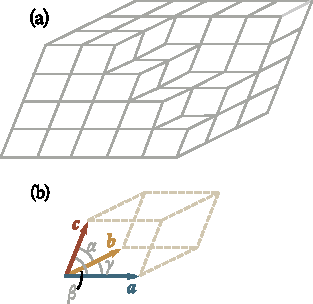
\includegraphics[scale=1]{figures/ch_13/fig_13_1.pdf}
			\caption[]{}
			\label{fig:13_1}
		\end{center}
	\end{minipage}
	\hspace{-0.05cm}
	\begin{minipage}[t]{0.5\linewidth}
		\begin{center}
			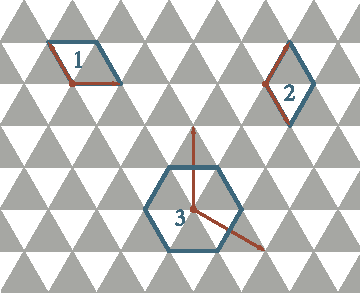
\includegraphics[scale=1]{figures/ch_13/fig_13_2.pdf}
			\caption[]{}
			\label{fig:13_2}
		\end{center}
	\end{minipage}
	\vspace{-0.4cm}
\end{figure}

%An elementary cell can be selected in various ways. This is illustrated in \fig{13_2} using an example of a plane structure. The facing of a wall with alternating light and dark triangular tiles can be obtained by repeating different cells many times in two directions (see, for example, cells $1$, $2$, and $3$; the arrows show the directions in which the cells are repeated). Cells $1$ and $2$ are distinguished by including the minimum number of structural elements (one light and one dark tile each). A crystal cell including the smallest number of atoms characterizing the chemical composition of a crystalline substance (for example, one oxygen atom and two hydrogen atoms for an ice crystal) is known as a \textbf{primitive cell}. It is customary practice, however, to select an elementary cell having a greater number of atoms, but with the same symmetry as the entire crystal, instead of a primitive cell. Thus, the plane structure depicted in \fig{13_2} coincides with itself when rotated through \SI{120}{\degree} about any axis at right angles to it that passes through an apex of a tile. Elementary cell $3$ has the same property. Cells $1$ and $2$ have a smaller degree of symmetry: they coincide with themselves only when rotated through \SI{360}{\degree}.

Có thể chọn ô sơ cấp theo nhiều cách khác nhau. Điều đó được chỉ rõ trên \fig{13_2} về thí dụ của một cấu trúc phẳng. Ta có thể thu được hình ảnh trên một bức tường gồm nhiều tấm tam giác sáng tối xen kẽ nhau bằng cách lặp đi lặp lại nhiều lần những ô khác nhau theo hai hướng (xem, chẳng hạn, các ô $1$, $2$, và $3$; các hướng mà ta lặp lại ở các ô được chỉ rõ bằng các mũi tên). Các ô $1$ và $2$ có đặc điểm là chúng chứa một số tối thiểu các yếu tố cấu trúc (mỗi ô chứa một tấm sáng và một tấm tối). Một ô tinh thể chứa một số tối thiêu nguyên tử đặc trưng cho thành phần hoá học của chất kết tinh (chẳng hạn, đối với tinh thể nước đá, có một nguyên tử oxy \iffalse oxygen\fi và hai nguyên tử hydro\iffalse hydrogen\fi) gọi là một \textbf{ô gốc}. Tuy vậy, thay cho ô gốc người ta thường chọn một ô sơ cấp có một số khá lớn nguyên tử, nhưng có cùng tính đối xứng giống như toàn bộ tinh thể. Chẳng hạn, cấu trúc phẳng vẽ trên \fig{13_2} sẽ trùng với chính nó khi quay \SI{120}{\degree} quanh bất kỳ một trục nào vuông góc với nó và đi qua đỉnh của một tấm. Ô sơ cấp số $3$ cũng có tính chất tương tự vậy. Ô $1$ và $2$ có bậc đối xứng thấp hơn: chúng trùng với chính nó chỉ khi quay \SI{360}{\degree}.

%\section{Classification of Crystals}\label{sec:13_2}

\section{Phân loại các tinh thể}\label{sec:13_2}

%A crystal lattice can have different kinds of symmetry. By the symmetry of a crystal lattice is meant its property to coincide with itself upon certain displacements in space.

Mạng tinh thể có thể có những dạng đối xứng khác nhau. Ta hiểu tính đối xứng của một mạng tinh thể là tính chất của mạng có thể trùng với chính nó trong một vài dịch chuyển không gian.

%Every lattice has translation symmetry first of all, \ie, it coincides with itself upon displacement over the translation period\footnote{When considering the symmetry of a lattice, the finite dimensions of the crystal are disregarded, and the lattice is considered to be infinite.}. Among the other kinds of symmetry, we shall note symmetry with respect to rotations about certain axes, and also to mirror reflection relative to definite planes.

Mỗi mạng tinh thể trước hết có tính đối xứng tịnh tiến, tức là nó sẽ trùng với chính nó trong sự dịch chuyển (tịnh tiến) một khoảng bằng chu kỳ trùng lặp \footnote{Khi xét tính đối xứng của một mạng tinh thể ta bỏ qua kích thước cụ thể của tinh thể và coi mạng như là vô hạn.}. Trong số những dạng đối xứng khác ta chú ý tới sự đối xứng đối với các phép quay quanh những trục nào đó, và cả đối với sự phản xạ gương đối với những mặt phẳng xác định.

%If a lattice coincides with itself when rotated about an axis through the angle $2\pi/n$ (consequently, the lattice coincides with itself $n$ times in one complete revolution about the axis), then this axis is called an \textbf{axis of symmetry} of the $n$-th order. It can be shown that apart from the trivial axis of the first order, only axes of symmetry of the second, third, fourth, and sixth orders are possible. Examples of structures having such axes of symmetry are shown schematically in \fig{13_3} (the empty circles, filled circles, and crosses signify atoms of different species).

Nếu mạng tinh thể trùng với chính nó khi quay quanh một trục nào đó một góc $2\pi/n$ (do đó, khi quay đúng một vòng quanh trục, mạng trùng với chính nó $n$ lần), thì trục này được gọi là các \textbf{trục đối xứng bậc $n$}. Có thể chứng minh rằng, ngoài trục bậc $1$ tầm thường, chỉ có thể có những trục đối xứng bậc $2$, bậc $3$, bậc $4$ và bậc $6$. Những thí dụ về các cấu trúc có các trục đối xứng như vậy được vẽ theo kiểu sơ đồ trên \fig{13_3} (những vòng tròn trắng, vòng tròn đen và những chữ thập nhỏ ký hiệu cho những nguyên tử thuộc những loại khác nhau).

\begin{figure}[!htb]
	\begin{center}
		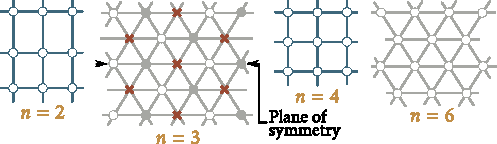
\includegraphics[scale=1.1]{figures/ch_13/fig_13_3.pdf}
		\caption[]{}
		\label{fig:13_3}
	\end{center}
	\vspace{-0.8cm}
\end{figure}

%If a lattice coincides with itself when reflected in a certain plane as in a mirror, this plane is defined as a \textbf{plane of symmetry}. An example of a plane of symmetry is also shown in \fig{13_3}.

Khi phản xạ gương những mặt phẳng mà qua đó mạng tinh thể trùng với chính nó gọi là những \textbf{mặt phẳng đối xứng}. Thí dụ về mặt phẳng đối xứng được vẽ trên \fig{13_3}.

%The different kinds of symmetry are called \textbf{elements of symmetry} of a crystal lattice. There are other elements of symmetry in addition to axes and planes, but we shall not consider them here, however.

Những dạng đối xứng khác nhau được gọi là những \textbf{yếu tố đối xứng} của mạng tinh thể. Ngoài các trục đối xứng và các mặt đối xứng, còn có thể có những yếu tố đối xứng khác nữa nhưng chúng ta sẽ không xét đến.

%A crystal lattice, as a rule, has several kinds of symmetry at a time. Not any combination of the elements of symmetry is possible, however. The prominent Russian scientist Yevgraf Fedorov (1853-1919) showed that $230$ combinations of the symmetry elements are possible. These combinations are called \textbf{space groups}. They are divided according to features of symmetry into $32$ classes. Finally, with respect to the shape of the elementary cell, all crystals are divided into seven \textbf{crystallographic systems}, each of which includes several classes of symmetry.

Một mạng tinh thể bao giờ cũng có đồng thời một vài dạng đối xứng. Tuy nhiên, không thể tổ hợp các yếu tố đối xứng với nhau một cách tuỳ tiện được. Nhà bác học Nga nổi tiếng Yevgraf Fedorov (1853-1919) đã chứng minh rằng chỉ có thể có $230$ tổ hợp các yếu tố đối xứng gọi là những \textbf{nhóm không gian}. $230$ nhóm không gian đó lại được chia thành $32$ lớp dựa vào các dấu hiệu đối xứng. Cuối cùng, dựa vào hình dạng của các ô sơ cấp, người ta lại chia tất cả các tinh thể thành bẩy \textbf{hệ tinh thể}, mỗi hệ bao gồm một vài lớp đối xứng.

%The crystallographic systems are arranged in the order of growth of their symmetry as follows.

Các hệ tinh thể được sắp xếp như sau theo thứ tự tính đối xứng tăng dần.
\begin{enumerate}[1.]

    %   \item \textbf{Triclinic System.} For this system, $a\neq b\neq c$; $\alpha\neq\beta\neq\gamma$. An elementary cell has the form of an oblique parallelepiped.

	\item \textbf{Hệ tam tà.} Đặc điểm của hệ này là $a\neq b\neq c$; $\alpha\neq\beta\neq\gamma$. Ô sơ cấp có dạng một hình hộp xiên.

    %	\item \textbf{Monoclinic System.} It has two right angles, while the third angle (usually the angle $\beta$) is not a right one. Hence, $a\neq b\neq c$; $\alpha=\gamma=\SI{90}{\degree}, \beta\neq\SI{90}{\degree}$. An elementary cell has the form of a right prism with a parallelogram as its base (\ie, the form of a right parallelepiped).

	\item \textbf{Hệ đơn tà.} Hệ có hai góc vuông, còn góc thứ ba khác với góc vuông (người ta thường ký hiệu góc này là $\beta$). Do đó $a\neq b\neq c$; $\alpha=\gamma=\SI{90}{\degree}, \beta\neq\SI{90}{\degree}$.  Ô sơ cấp có dạng một lăng trụ thẳng, mặt đáy của nó là một hình bình hành (tức là ô sơ cấp có hình dạng một hình hộp thẳng).

 %	\item \textbf{Rhombic System.} All the angles are right ones, all the edges are different: $a\neq b\neq c$; $\alpha=\beta=\gamma=\SI{90}{\degree}$. An elementary cell has the form of a rectangular parallelepiped.

	\item \textbf{Hệ thoi.} Tất cả các góc đều là góc vuông, tất cả các cạnh đều khác nhau: $a\neq b\neq c$; $\alpha=\beta=\gamma=\SI{90}{\degree}$. Ô sơ cấp có dạng một hình hộp chữ nhật.

%	\item \textbf{Tetragonal System.} All the angles are right ones, two edges are equal: $a=b\neq c$; $\alpha=\beta=\gamma=\SI{90}{\degree}$. An elementary cell has the form of a right prism with a square base.

	\item \textbf{Hệ tứ giác.} Tất cả các góc đều là góc vuông; hai cạnh bằng nhau: $a=b\neq c$; $\alpha=\beta=\gamma=\SI{90}{\degree}$. Ô sơ cấp có dạng một lăng trụ thẳng mà đáy là một hình vuông.

%	\item \textbf{Rhombohedral (or Trigonal) System.} All the edges are equal, all the angles are also equal and are other than right ones: $a=b=c$; $\alpha=\beta=\gamma\neq\SI{90}{\degree}$. An elementary cell has the form of a cube deformed by compression or tension along a diagonal.

	\item \textbf{Hệ quả trám (hệ tam giác).} Tất cả các cạnh đều bằng nhau, tất cả các góc cũng bằng nhau nhưng khác góc vuông: $a=b=c$; $\alpha=\beta=\gamma\neq\SI{90}{\degree}$. Ô sơ cấp có dạng một hình lập phương biến dạng do sự nén hoặc kéo dãn dọc theo một đường chéo.

%	\item \textbf{Hexagonal System.} The edges and the angles between them comply with the conditions $a=b\neq c$; $\alpha=\beta=\SI{90}{\degree}, \gamma=\SI{120}{\degree}$. 	Three elementary cells brought together as shown in \fig{13_4} form a regular hexagonal prism.

	\item \textbf{Hệ lục giác.} Các cạnh và góc giữa các cạnh này thoả mãn các điều kiện sau: $a=b\neq c$; $\alpha=\beta=\SI{90}{\degree}, \gamma=\SI{120}{\degree}$. Nếu ta vẽ đồng thời ba ô sơ cấp như ở \fig{13_4}, ta sẽ thu được một hình lăng trụ lục giác đều.

%	\item \textbf{Cubic System.} All the edges are equal, all the angles are right ones: $a=b=c$; $\alpha=\beta=\gamma=\SI{90}{\degree}$. An elementary cell has the form of a cube.

	\item \textbf{Hệ lập phương.} Tất cả các cạnh đều bằng nhau, tất cả các góc đều là góc vuông: $a=b=c$; $\alpha=\beta=\gamma=\SI{90}{\degree}$. Ô sơ cấp có dạng một hình lập phương.
\end{enumerate}

%\section{Physical Kinds of Crystal Lattices}\label{sec:13_3}

\section{Các loại mạng tinh thể phân theo lý tính}\label{sec:13_3}

%Four kinds of crystal lattices and accordingly four kinds of crystals are distinguished depending on the nature of the particles at the lattice points and on the nature of the forces of interaction between the particles. They are ionic, atomic, metallic, and molecular crystals.

Tuỳ theo bản chất của các hạt nằm ở các nút mạng tinh thể và tuỳ theo đặc tính của các lực tương tác giữa các hạt, người ta phân ra bốn loại mạng tinh thể và một cách tương ứng bốn loại tinh thể: các tinh thể ion, nguyên tử, kim loại và phân tử.

%\textbf{1. Ionic Crystals.} Ions of opposite signs inhabit the lattice points. The forces of interaction between them are mainly electrostatic (Coulomb). The bond due to the electrostatic forces of attraction between oppositely charged ions is called a \textbf{heteropolar} (or \textbf{ionic}) bond.

\textbf{1. Các tinh thể ion.} Ở các nút của mạng tinh thể có các ion trái dấu. Lực tương tác giữa chúng về cơ bản là các lực tĩnh điện (lực Coulomb). Liên kết do lực hút tĩnh điện giữa các ion điện tích trái dấu gây ra gọi là \textbf{liên kết dị cực} (hay \textbf{liên kết ion}).

%A typical example of an ionic lattice is that of table salt (\ce{NaCl}) shown in \fig{13_5}. It belongs to the cubic system. The white circles depict the positively charged sodium ions, and the black circles the negative chloride ions. A glance at the figure shows that the closest neighbours of an ion of a given sign will be ones of the opposite sign. In the gaseous state, \ce{NaCl} consists of molecules in which sodium ions are combined with chloride ones in pairs. The group of an \ce{Na} ion and a \ce{Cl} ion forming a molecule loses its isolated existence in a crystal. An ionic crystal consists of ions, and not of molecules. The entire crystal can be considered as a single giant molecule.

Thí dụ điển hình về mạng tinh thể ion là mạng tinh thể muối ăn (\ce{NaCl}) vẽ trên \fig{13_5}. Mạng này thuộc hệ lập phương. Các vòng tròn trắng biểu hiện cho các ion natri \iffalse ion sodium \fi mang điện tích dương, các vòng tròn đen biểu diễn các ion âm clo\iffalse ion chloride\fi. Trên hình vẽ ta thấy những ion lân cận của một ion nào đó lại là những ion trái dấu. Ở trạng thái khí, \ce{NaCl} cấu tạo bởi những phân tử, trong đó các ion natri và ion clo liên kết với nhau thành từng cặp, Trong tinh thể, việc nhóm các ion \ce{Na} và \ce{Cl} thành phân tử mất hết ý nghĩa đặc biệt. Tinh thể ion không cấu tạo bằng những phân tử mà bằng những ion. Có thể coi toàn bộ tinh thể như một phân tử khổng lồ.

\begin{figure}[!htb]
	\begin{minipage}[t]{0.5\linewidth}
		\begin{center}
			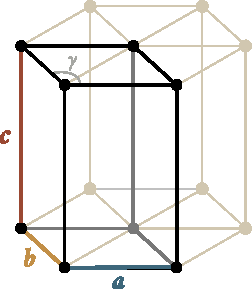
\includegraphics[scale=1.0]{figures/ch_13/fig_13_4.pdf}
			\caption[]{}
			\label{fig:13_4}
		\end{center}
	\end{minipage}
	\hspace{-0.05cm}
	\begin{minipage}[t]{0.5\linewidth}
		\begin{center}
			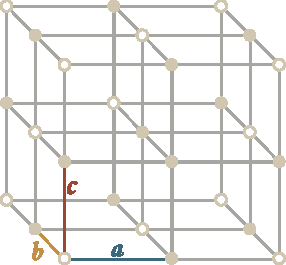
\includegraphics[scale=1.0]{figures/ch_13/fig_13_5.pdf}
			\caption[]{}
			\label{fig:13_5}
		\end{center}
	\end{minipage}
	\vspace{-0.4cm}
\end{figure}

%\textbf{2. Atomic Crystals.} The lattice points accommodate neutral atoms. The bond between neutral atoms in a crystal (and also in a molecule) is called \textbf{homopolar} (or \textbf{covalent}). The forces of interaction with a homopolar bond are also of an electrical (but not of a Coulomb) nature. These forces can be explained only on the basis of quantum mechanics.

\textbf{2. Các tinh thể nguyên tử.} Tại các nút của mạng tinh thể có các nguyên tử trung hoà. Trong tinh thể (và cả trong phân tử) liên kết nối các nguyên tử trung hoà lại được gọi là \textbf{liên kết đồng lực} (hoặc \textbf{liên kết cộng hoá trị}). Các lực tương tác trong liên kết đồng cực cũng có tính chất điện (nhưng không phải các lực Coulomb). Ta chỉ có thể giải thích được các lực đó trên cơ sở của cơ học lượng tử.

%A homopolar bond is produced by electron pairs. This signifies that one electron from each atom participates in setting up a bond between two atoms. For this reason, a homopolar bond has a directed nature. In a heteropolar bond, each ion acts on all the ions that are sufficiently close to it. In a homopolar bond, the action is directed toward the atom with which the given one shares an electron pair. A homopolar bond can be set up only by valence electrons, whose bond to the atom is the weakest. Since each electron can set up a bond with only one atom, the number of bonds which a given atom can participate in (the number of neighbours with which it can be bound) equals its valence.

Liên kết đồng cực được thực hiện bằng những cặp electron. Điều đó có nghĩa là để đảm bảo mối liên kết giữa hai nguyên tử, thì mỗi nguyên tử có một electron tham gia vào liên kết đó. Vì lý do đó, liên kết đồng cực có tính chất định hướng. Trong liên kết dị cực, mỗi ion tác động lên tất cả những ion nằm tương đối gần nó. Trong liên kết đồng cực, tác động được hướng tới nguyên tử nào có chung với nguyên tử đã cho một cặp electron tương thích. Chỉ có những electron hoá trị mới có thể thực hiện được liên kết đồng cực; đó là những electron có liên kết yếu nhất với nguyên tử. Vì mỗi electron chỉ có thể đảm bảo được một liên kết với một nguyên tử, nên số liên kết mà một nguyên tử đã cho có thể tham gia vào (số nguyên tử lân cận có liên kết với nguyên tử đã cho) phải bằng hoá trị của nó.

%Typical examples of atomic crystals are diamond and graphite. The chemical nature of these two substances is the same (they are both constructed of carbon atoms), but they differ in the structure of their crystals. Figure~\ref{fig:13_6}a shows a diamond lattice, and \fig{13_6}b a graphite one. This example clearly shows how the crystal structure of a substance affects its properties.

Các thí dụ điển hình của các tinh thể nguyên tử có thể là kim cương và graphite. Cả hai chất này đều đồng nhất với nhau về bản chất hoá học (chúng đều được cấu tạo từ các nguyên tử cacbon\iffalse carbon\fi), nhưng chúng có cấu tạo tinh thể khác nhau. Trên hình~\ref{fig:13_6}a ta vẽ mạng kim cương, trên \fig{13_6}b ta vẽ mạng graphite. Trong thí dụ này ta thấy rõ ảnh hưởng của cấu trúc tinh thể đến các tính chất của các chất.

%The typical semiconductors----germanium (\ce{Ge}) and silicon (\ce{Si}) have the same kind of lattice as diamond (a diamond-type lattice). This lattice is characterized by each atom being surrounded by four neighbours at an equal distance from it located at the corners of a regular tetrahedron. Each of the four valence electrons belongs to an electron pair joining this atom with one of its neighbours.

Các chất bán dẫn điển hình như germani \iffalse germanium\fi (\ce{Ge}) và silic \iffalse silicon\fi (\ce{Si}) cũng có mạng như kim cương (mạng kiểu kim cương). Đối với mạng này, điểm đặc trưng là mỗi nguyên tử được bao quanh bởi bốn nguyên tử lân cận cách đều nó, nằm tại các đỉnh của mỗi tứ diện đều. Mỗi electron trong số bốn electron hoá trị sẽ tham gia vào một cặp electron liên kết nguyên tử đã cho với một nguyên tử lân cận nó.

\begin{figure}[!htb]
	\begin{center}
		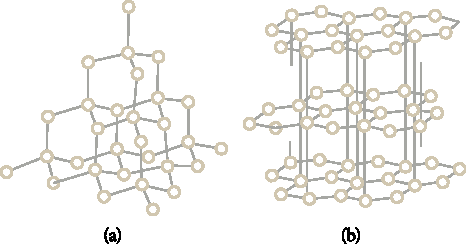
\includegraphics[scale=1.0]{figures/ch_13/fig_13_6.pdf}
		\caption[]{}
		\label{fig:13_6}
	\end{center}
	\vspace{-0.4cm}
\end{figure}

\begin{figure}[!htb]
	\begin{center}
		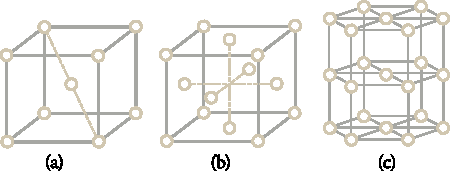
\includegraphics[scale=1.0]{figures/ch_13/fig_13_7.pdf}
		\caption[]{}
		\label{fig:13_7}
	\end{center}
	\vspace{-0.8cm}
\end{figure}

%\textbf{3. Metallic Crystals.} Positive ions of the metal are located at all the lattice points. Electrons that detached themselves from the atoms when ions were formed move chaotically between the latter similar to the molecules of a gas. These electrons play the part of a ``cement'' keeping the positive ions together, otherwise the lattice would fall apart under the action of the forces of repulsion between the ions. At the same time, the electrons, in turn, are retained by the ions within the crystal lattice and cannot leave it.

\textbf{3. Những tinh thể kim loại.} Tất cả các nút của mạng tinh thể có những ion dương kim loại. Giữa chúng có những electron chuyển động hỗn loạn giống như những phân tử khí; những electron này bị tách khỏi các nguyên tử khi tạo thành các ion. Những electron này đóng vai trò của ``xi măng'' gắn các ion dương lại với nhau; trong trường hợp ngược lại, mạng sẽ bị rã ra dưới tác dụng của các lực đẩy giữa các ion. Đồng thời các electron cũng lại bị các ion giữ lại trong phạm vi của mạng tinh thể, không cho chúng có thể thoát ra ngoài.

%Most metals have lattices of one of three kinds: the cubic volume-centred (\fig{13_7}a), the cubic face-centred (\fig{13_7}b), and the so-called hexagonal close-packed lattice (\fig{13_7}c). The latter is a hexagonal lattice with the ratio $c/a$ equal to $\sqrt{8/3}$. The cubic face-centred and the hexagonal close-packed lattices correspond to the closest packing of identical spheres.

Phần lớn các kim loại có mạng thuộc một trong ba kiểu: lập phương thể tâm (\fig{13_7}a), lập phương diện tâm (\fig{13_7}b), và mạng mà người ta gọi là mạng lục giác chặt (\fig{13_7}c). Mạng lục giác chặt là mạng có tỷ số $c/a$ bằng $\sqrt{8/3}$. Mạng lập phương diện tâm và mạng lục giác chặt ứng với sự bó chặt nhất những quả cầu giống nhau.

%\textbf{4. Molecular Crystals.} Molecules with a definite orientation are located at the lattice points. The forces binding together the molecules in a crystal are of the same nature as the forces of attraction between molecules leading to gases deviating from ideal ones in their properties. This is why they are called \textbf{van der Waals forces}. Molecular lattices are formed, for example, by the following substances: \ce{H2}, \ce{N2}, \ce{02}, \ce{C02}, \ce{H20}. Thus, ordinary ice, and also the so-called dry ice (solid carbon dioxide) are molecular crystals.

\textbf{4. Những tinh thể phân tử.} Tại các nút mạng tinh thể có những phân tử định hướng một cách xác định. Những lực liên kết giữa các phân tử trong tinh thể có cùng bản chất với các lực hút giữa các phân tử; các lực này đã làm cho các chất khí thực khác với khí lý tưởng. Vì lý do đó, các lực này được gọi là \textbf{lực van der Waals}. Những chất sau đây, chẳng hạn, lập thành mạng tinh thể phân tử: \ce{H2}, \ce{N2}, \ce{02}, \ce{C02}, \ce{H20}. Vì vậy, nước đá thông thường (và cả cacbonic rắn\iffalse carbon dioxide\fi) là những tinh thể phân tử.

%\section{Defect in Crystals}\label{sec:13_4}

\section{Các khuyết tật trong các tinh thể}\label{sec:13_4}

%Defects in crystals are violations of an ideal crystalline structure. Such a violation may consist in the absence of an atom at a lattice point (a vacancy), in the presence of a foreign atom (an impurity atom) instead of an atom of the given substance (a host atom), in the introduction of a surplus atom (host or foreign) into the interstice. Such defects are called \textbf{point} ones. They cause violations in the regularity of a lattice extending over a distance of the order of several periods.

Ta gọi những sai lệch trong cấu trúc tinh thể lý tưởng là những khuyết tật của các tinh thể. Sai lệch đó có thể là sự khuyết một nguyên tử ở nút mạng (chỗ khuyết), sự thay thế một nguyên tử của chất đã cho (nguyên tử của mình) bằng một nguyên tử lạ (nguyên tử tạp chất), sự đưa thêm một nguyên tử thừa (nguyên tử của mình hoặc nguyên tử lạ) vào khoảng không gian giữa các nút. Những khuyết tật loại này được gọi là những \textbf{khuyết tật điểm}. Chúng gây ra những sai lệch về sự đều đặn của mạng trên một vùng có kích thước khoảng một vài chu kỳ.

%In addition to point defects, there are also defects concentrated near certain lines. They are called \textbf{linear defects} or \textbf{dislocations}. Defects of this kind violate the regular alternation of the crystal planes. The simplest defects of this kind are \textbf{edge} and \textbf{screw} dislocations.

Ngoài những khuyết tật điểm, còn có những khuyết tật tập trung gần những đường nào đó. Ta gọi chúng là những \textbf{khuyết tật dài} hoặc \textbf{lệch mạng}. Những khuyết tật dạng này làm hỏng sự xen kẽ đều đặn của các mặt phẳng tinh thể. Những dạng lệch mảng đơn giản nhất loại này là  \textbf{lệch mạng bờ} và \textbf{lệch mạng xoắn ốc}.

%An edge dislocation is due to a surplus crystal half-plane inserted between two adjacent layers of atoms (\fig{13_8}). The edge of this half-plane forms a dislocation of the given kind. The dislocation line is the straight line denoted by the symbol $\perp$ at right angles to the plane of the drawing.

Lệch mạng bờ được gây ra do một nửa mặt phẳng tinh thể thừa bị đẩy vào giữa hai lớp nguyên tử cạnh nhau (\fig{13_8}). Bờ của nửa mặt phẳng đó tạo ra sự lệch mạng thuộc dạng đã cho. Đường lệch mạng là đường thẳng vuông góc với mặt phẳng hình vẽ và được đánh dấu bằng dấu $\perp$.

%A screw dislocation can be presented as a result of cutting a crystal along a half-plane and the following shifting of the lattice portions at different sides of the cut toward each other over a distance of one period (\fig{13_9}). The internal edge of the cut forms a screw dislocation (see the dash line in the figure). A crystal with a screw dislocation actually consists of a single crystal plane that is curved along a helical surface (such a surface is called a helicoid). The dislocation line coincides with the axis of the screw or helix. The crystal plane is displaced by one period each time it circumvents this line.

Có thể coi lệch mạng xoắn ốc như kết quả của việc cắt tinh thể theo một nửa mặt phẳng, tiếp sau đó là đẩy trượt hai phần của mạng nằm về hai phía khác nhau của mặt phẳng cắt theo chiều ngược nhau đi một khoảng bẳng một chu kỳ (\fig{13_9}). Bờ trong của vết cắt tạo thành lệch mạng xoắn ốc (xem đường thẳng chấm chấm trên hình vẽ). Tinh thể có lệch mạng xoắn ốc thực tế chỉ có một mặt phẳng tinh thể bị uốn theo bề mặt của một đinh ốc (mặt này gọi là mặt đinh ốc). Đường lệch mạng trùng với trục của đinh ốc. Sau mỗi vòng quay chung quanh đường đó, mặt phẳng tinh thể dịch đi một chu kỳ. 

\begin{figure}[!htb]
	\begin{minipage}[t]{0.5\linewidth}
		\begin{center}
			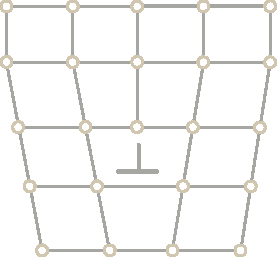
\includegraphics[scale=1.0]{figures/ch_13/fig_13_8.pdf}
			\caption[]{}
			\label{fig:13_8}
		\end{center}
	\end{minipage}
	\hspace{-0.05cm}
	\begin{minipage}[t]{0.5\linewidth}
		\begin{center}
			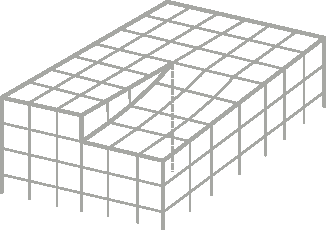
\includegraphics[scale=1.0]{figures/ch_13/fig_13_9.pdf}
			\caption[]{}
			\label{fig:13_9}
		\end{center}
	\end{minipage}
	\vspace{-0.4cm}
\end{figure}

%We have considered the two simplest (extreme) kinds of dislocations. In both cases, the dislocation lines are straight. In the general case, these lines may be curved.

Chúng ta đã xét hai dạng lệch mảng đơn giản nhất (hai dạng giới hạn). Trong cả hai trường hợp những đường lệch mạng là những đường thẳng. Trong trường hợp tổng quát, những đường lệch mạng có thể là những đường cong.

%Defects greatly affect the physical properties of crystals, including their strength. In particular, dislocations are the reason why the plastic deformation\footnote{A plastic deformation is one that remains after the stress causing it is removed.} of real crystals occurs under the action of stresses that are several orders of magnitude smaller than the stress calculated for ideal crystals.

Những khuyết tật có ảnh hướng lớn đến các tính chất vật lý của các tinh thể, trong đó có cả độ bền của chúng. Đặc biệt, các lệch mạng là nguyên nhân làm cho biến dạng dẻo\footnote{Biến dạng dẻo là biến dạng được giữ nguyên sau khi đã bỏ đi lực gây biến dạng.} của các tinh thể thực xuất hiện dưới tác động của lực gây biến dạng nhỏ hơn một vài bậc so với tác động được tính toán đối với các tinh thể lý tưởng.

%Shear along the atomic layers readily occurs in the monocrystals of metals. Do not imagine this process in such a way that all the atoms of a layer are displaced simultaneously as a single whole. Actually, the atoms jump over into their new positions in small groups, sequentially. Such a sequential movement of the atoms can be presented as a dislocation movement. The latter requires stresses much smaller than those needed for the displacement of an entire atomic layer at a time. Figure~\ref{fig:13_10} shows the consecutive steps of the process occurring in a crystal under the action of the forces causing the shear. The initially present dislocation under the action of the stresses set up in the crystal moves along the latter. This movement is attended by sequential displacement of the atoms in the layer above the dislocation relative to the atoms of the layer under it.

Ở các đơn tinh thể kim loại dễ dàng xuất hiện biến dạng trượt dọc theo các lớp nguyên tử. Ta không nên hình dung trong quá trình này tất cả các nguyên tử của một lớp xê dịch đồng thời như một toàn thể. Thực tế thì từng nhóm nhỏ nguyên tử lần lượt nhảy sang vị trí mới. Sự dịch chuyển lần lượt của các nguyên tử có thể được hình dung sự như chuyển động của lệch mạng. Để làm di chuyển một lệch mạng chỉ cần một lực nhỏ hơn rất nhiều so với việc làm dịch chuyển ngay một lúc toàn bộ một lớp nguyên tử. Trên hình~\ref{fig:13_10} có vẽ những giai đoạn kế tiếp nhau của một quá trình xảy ra trong một tinh thể dưới tác dụng của những lực gây ra biến dạng trượt. Thoạt tiên lệch mạng có được dưới tác động của những ứng lực xuất hiện trong tinh thể sẽ dịch chuyển dọc theo tinh thể. Dịch chuyển này kèm theo sự trượt lần lượt của các nguyên tử trong lớp nằm trên chỗ lệch mạng so với các nguyên tử trong lớp nằm dưới chỗ lệch mạng.

%Dislocation movements are prevented by the presence of other defects in a crystal, for example, by the presence of impurity atoms. Dislocations are also inhibited when they intersect. If the number of dislocations and other defects in a crystal is small, the dislocations spread virtually without hindrance. As a result, the resistance to shear will not be great. An increase in the density of the dislocations and a growth in the concentration of the impurities lead to great inhibition of the dislocations and stopping of their spreading. As a result, the strength of the material grows. For example, the strength of iron is increased by dissolving carbon atoms in it (steel is such a solution).

Sự có mặt của các khuyết tật khác trong tinh thể, chẳng hạn sự có mặt của các nguyên tử tạp chất, sẽ ngăn cản sự dịch chuyển của các lệch mạng. Các lệch mạng cũng bị hãm lại khi chúng giao nhau. Nếu số những lệch mạng và những khuyết tật khác nhau trong tinh thể không lớn thì những lệch mạng di chuyển gần như tự do. Kết quả là sự cản trở biến dạng trượt sẽ nhỏ. Tăng mật độ của những lệch mạng và tăng nồng độ của tạp chất sẽ đưa đến sự hãm rất mạnh chuyển động của các lệch mạng và đưa đến sự ngừng hẳn chuyển động của chúng. Kết quả là độ bền của vật liệu sẽ tăng lên. Chẳng hạn, ta sẽ làm tăng độ bền của sắt nếu hoà tan trong nó các nguyên tử cacbon (dung dịch đó chính là thép). 

%Plastic deformation is attended by the destruction of the crystal lattice and the formation of a great number of defects preventing the spreading of the dislocations. This explains why metals are hardened upon their cold working.

Biến dạng dẻo thường kèm theo sự phá huỷ mạng tinh thể và tạo thành một lượng lớn các khuyết tật ngăn cản sự di chuyển của các lệch mạng. Điều đó giải thích tại sao khi gia công nguội các vật liệu trở nên bền chắc.

\begin{figure}[!htb]
	\begin{center}
		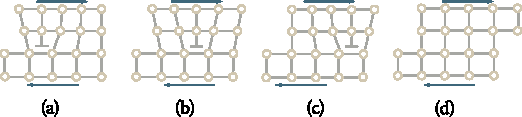
\includegraphics[scale=1.0]{figures/ch_13/fig_13_10.pdf}
		\caption[]{}
		\label{fig:13_10}
	\end{center}
	\vspace{-0.8cm}
\end{figure}

%A screw dislocation often appears in the course of the growth of a crystal from a solution or melt. The capture of an atom by a smooth flat crystal surface is less profitable from the energy viewpoint and is therefore less probable than the attachment of an atom to a step on the surface of a crystal with a screw dislocation. This is why it is preferable practice to grow crystals with a screw dislocation built into them. New atoms attach themselves to the edge of the step, owing to which the crystal grows along a spiral.

Lệch mạng xoắn ốc thường xuất hiện trong quá trình nuôi các tinh thể từ dung dịch hoặc từ chất nóng chảy. Việc bắt thêm một nguyên tử bởi một mặt tinh thể phẳng, nhẵn thì không thuận lợi về phương diện năng lượng, do đó xác suất xảy ra nhỏ hơn so với việc gắn thêm một nguyên tử vào chỗ gấp khúc trên mặt tinh thể có lệch mạng xoắn. Vì vậy các tinh thể thường lớn lên với lệch mạng xoắn ở bên trong. Những nguyên tử mới được gắn thêm vào bờ của chỗ gấp khúc, do đó sự lớn lên của tinh thể thường xảy ra theo đường hình xoắn ốc.

%\section{Heat Capacity of Crystals}\label{sec:13_5}

\section{Nhiệt dung của các tinh thể}\label{sec:13_5}

%The location of particles at the points of a crystal lattice corresponds to a minimum of their mutual potential energy. When particles are displaced from their equilibrium position in any direction, a force appears that tends to return them to their initial position. As a result, oscillations of the particles begin. Oscillation in an arbitrary direction can be represented as the superposition of oscillations in three mutually perpendicular directions. Therefore, three vibrational degrees of freedom should be ascribed to every particle in a crystal.

Sự sắp xếp các hạt ở các nút của mạng tinh thể ứng với giá trị cực tiểu của thế năng tương tác với chúng. Khi các hạt bị xê dịch khỏi vị trí cân bằng về bất kỳ hướng nào cũng xuất hiện một lực có xu hướng kéo hạt về vị trí ban đầu, do đó xuất hiện sự dao động của hạt. Sự dao động dọc theo bất kỳ phương nào cũng có thể coi như tổng hợp của những dao động dọc theo ba phương vuông góc lẫn nhau. Vì vậy người ta phản gán cho mỗi hạt trong tinh thể ba bậc tự do về dao động.

%We learned in Sec.~\ref{sec:11_5} that an energy equal to two halves of $kT$---one half in the form of kinetic and the other in the form of potential energy---falls on the average to each vibrational degree of freedom. Consequently, an energy equal to $3kT$ falls on the average to every particle---every atom in an atomic lattice, every ion in an ionic or metallic lattice\footnote{Matters are more complicated for molecular crystals. The molecules in addition to translational oscillations also perform torsional oscillations. Apart from this, the atoms oscillate inside the molecules.}. We can find the energy of a mole of a substance in the crystalline state by multiplying the mean energy of one particle by the number of particles at the points of the crystal lattice. The latter number coincides with the Avogadro constant $\ab{N}{A}$ only for chemically simple substances. For a diatomic substance such as \ce{NaCl}, the number of particles will be $2\ab{N}{A}$ because a mole of \ce{NaCl} contains $\ab{N}{A}$ atoms of \ce{Na} and $\ab{N}{A}$ atoms of \ce{Cl}, for a triatomic one it will be $3\ab{N}{A}$ and so on.

Trong phần~\ref{sec:11_5} ta thấy rằng ứng với mỗi bậc tự do về dao động trung bình có một năng lượng bằng hai nửa của $kT$: một dưới dạng động năng và một dưới dạng thế năng. Vì vậy ứng với một hạt, nghĩa là với mỗi nguyên tử trong mạng nguyên tử, mỗi ion trong mạng ion hay kim loại\footnote{Trong trường hợp các tinh thể phân tử thì vấn đề có phức tạp hơn. Các phân tử, ngoài những dao động tịnh tiến, còn thực hiện những dao động xoắn. Ngoài ra, lại còn sự dao động của các nguyên tử bên trong phân tử.}, trung bình có một năng lượng bằng $3kT$. Ta có thể tìm được năng lượng của một mol ở trạng thái kết tinh bằng cách nhân năng lượng trung bình của một hạt với số hạt nằm tại các nút của mạng tinh thể. Số hạt này chỉ trùng với số Avogadro $\ab{N}{A}$ trong trường hợp những chất đơn giản về phương diện hoá học. Chẳng hạn, trong trường hợp các chất có hai nguyên tử như \ce{NaCl}, số hạt sẽ bằng $2\ab{N}{A}$, vì rằng trong một mol \ce{NaCl} có chứa $\ab{N}{A}$ nguyên tử \ce{Na} và $\ab{N}{A}$ nguyên tử \ce{Cl}, với chất có ba nguyên tử thì số hạt sẽ bằng $3\ab{N}{A}$ và tương tự.

%Restricting ourselves to a consideration of chemically simple substances forming atomic or metallic crystals, we can write the following expression for the internal energy of a mole of a substance in the crystalline state:

Nếu chỉ giới hạn trong việc xét những chất đơn giản về phương diện hoá học cấu tạo nên những tinh thể nguyên tử hoặc tinh thể kim loại thì ta có thể viết biểu thức sau đây cho nội năng của một mol chất ở trạng thái kết tinh: 
\begin{equation*}
	\ab{U}{m} = \ab{N}{A} 3kT = 3RT.
\end{equation*}

%The increment of the internal energy corresponding to elevation of the temperature by one kelvin, according to \eqn{12_53}, equals the heat capacity at constant volume. Hence,

Theo \eqn{12_53}, độ tăng nội năng ứng với sự tăng nhiệt độ lên một độ bằng nhiệt dung trong quá trình đẳng tích. Do đó
\begin{equation}\label{eq:13_1}
	C_V = 3R.
\end{equation}

\noindent

%Since the volume of solids changes only slightly when they are heated, their heat capacity at constant pressure insignificantly differs from the heat capacity at constant volume; we can therefore assume that $C_p\approx C_V$ and speak simply of the heat capacity of a solid.

Vì rằng khi đun nóng, thể tích của các vật rắn thay đổi rất ít, nên nhiệt dung trong quá trình đẳng tích rất ít. Vì vậy, có thể đặt $C_p\approx C_V$ và có thể nói một cách đơn giản về nhiệt dung của một vật rắn.

%Thus, \eqn{13_1} states that the molar heat capacity of chemically simple bodies in the crystalline state is the same and equals $3R$. This statement is the content of the \textbf{Dulong and Petit law} established experimentally. This law is obeyed with quite a good approximation for many substances at room temperature. There are exceptions to this law, however. For example, diamond has a heat capacity of only about $0.7R$ at room temperature.

Vậy theo \eqn{13_1} nhiệt dung của một mol các chất đơn giản về phương diện hoá học ở trạng thái kết tinh là như nhau và bằng $3R$. Điều khẳng định này là nội dung của \textbf{định luật Dulong và Petit} đã được thiết lập bằng thực nghiệm. Một cách gần đúng, định luật này được thoả mãn đối với nhiều chất ở nhiệt độ phòng. Tuy nhiên, chẳng hạn kim cương ở nhiệt độ phòng có nhiệt dung chỉ bằng $0.7R$.

\begin{figure}[!htb]
	\begin{center}
		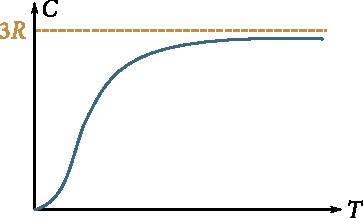
\includegraphics[scale=1.0]{figures/ch_13/fig_13_11.pdf}
		\caption[]{}
		\label{fig:13_11}
	\end{center}
	\vspace{-0.8cm}
\end{figure}

%Moreover, notwithstanding \eqn{13_1}, the heat capacity of crystals depends on the temperature, this dependence having the nature shown in \fig{13_11}. Near absolute zero, the heat capacity of all bodies is proportional to $T^3$, and only at a sufficiently high temperature characteristic of each substance does \eqn{13_1} begin to be obeyed. For most substances, this already occurs at room temperature. But for diamond the heat capacity only reaches the value of $3R$ at a temperature of about \SI{1000}{\degreeCelsius}.

Hơn nữa, trái với \eqn{13_1}, nhiệt dung của các tinh thể phụ thuộc vào nhiệt độ, trong đó sự phụ thuộc này có đặc điểm được nêu trên \fig{13_11}. Gần độ không tuyệt đối nhiệt dung của tất cả các vật tỷ lệ với $T^3$, và chỉ ở nhiệt độ khá cao đặc trưng cho mỗi chất, \eqn{13_1} mới được nghiệm đúng. Đối với phần lớn các chất điều kiện này đạt được ngay cả ở nhiệt độ phòng, nhưng đối với kim cương nhiệt dung chỉ đạt giá trị $3R$ ở nhiệt độ khoảng \SI{1000}{\degreeCelsius}.

%The strict theory of the heat capacity of solids proposed by A. Einstein and P. Debye takes into account, first, the quantization of the energy of vibrational motion (see Sec.~\ref{sec:11_5}). Second, the theory takes into account that the oscillations of the particles in a crystal lattice are not independent. This theory, which we shall set out in Volume 3, is in good agreement with experimental data. In particular, for high temperatures, it leads to \eqn{13_1}.

Lý thuyết chặt chẽ về nhiệt dung của vật rắn do A. Einstein và P. Debye xây dựng, trước hết tính đến sự lượng tử hoá năng lượng của chuyển động dao động (xem phần~\ref{sec:11_5}). Thứ hai là thuyết này tính đến sự kiện là dao động của các hạt ở trong mạng tinh thể không phải là độc lập. Lý thuyết này phù hợp tốt với những dữ kiện thực nghiệm. Đặc biệt ở những nhiệt độ cao, nó đưa đến \eqn{13_1}.
